%% ma: L12-B03-0015
%% lop: 12
%% chuong: 1
%% bai: 3
%% dang: 12.3.12
%% loai: TN4
%% muc: TH
%% dap_an: "A"
%% nguon: "(NBV)-ĐỀ SỐ 18-MỖI NGÀY 1 ĐỀ THI 2025.pdf (D18, MỖI NGÀY 1 ĐỀ - Đề số 18), Phần I Câu 7"
%% kien_thuc: "Bài 3 (tiệm cận đứng, tiệm cận ngang đọc từ bảng biến thiên)"
%% trang_thai: cho-duyet
%% ly_do: "Dạng mới đề xuất 12.3.12 (đếm số đường tiệm cận từ bảng biến thiên của hàm số xác định trên (-vô cùng; 0) trừ {-2}: x tiến tới 0 từ bên trái không cho tiệm cận ngang), chờ giáo viên duyệt."
%% ghi_chu: "Đáp án gốc A đúng (chỉ có tiệm cận đứng x = -2). Bảng gốc có cột x = 0 và +vô cùng với phần tô gạch (ngoài tập xác định); bản kho vẽ bảng dừng ở x = 0."
\begin{ex}
Cho hàm số $f(x)$ xác định trên $(-\infty;0)\setminus\{-2\}$ và có bảng biến thiên như sau. Đồ thị hàm số đã cho có tổng số đường tiệm cận ngang và tiệm cận đứng là
\begin{center}
\begin{tikzpicture}
  \tkzTabInit[lgt=1.6,espcl=2.6]{$x$/.8,$f'(x)$/.8,$f(x)$/2}{$-\infty$,$-2$,$0$}
  \tkzTabLine{,+,d,-,}
  \tkzTabVar{-/$-\infty$,+D+/$+\infty$/$1$,-/$0$}
\end{tikzpicture}
\end{center}
\choice{\True $1$}{$3$}{$0$}{$2$}
\loigiai{Vì $\lim\limits_{x\to-2^-}f(x)=+\infty$ nên đường thẳng $x=-2$ là tiệm cận đứng.

Hàm số chỉ xác định trên $(-\infty;0)\setminus\{-2\}$ và $\lim\limits_{x\to-\infty}f(x)=-\infty$, $\lim\limits_{x\to0^-}f(x)=0$ (đây không phải giới hạn khi $x\to\pm\infty$) nên đồ thị không có tiệm cận ngang.

Vậy đồ thị có đúng $1$ đường tiệm cận. Chọn A.}
\end{ex}
